\documentclass[a4paper,12pt]{paper}

\usepackage{mycommands}

% Worked-example layout: boxed problem statement followed by a solution.
\newcounter{example}
\renewenvironment{example}[1]{%  % the paper class already defines "example"
  \refstepcounter{example}%
  \begin{mdframed}[linewidth=1pt,innertopmargin=6pt,innerbottommargin=6pt]%
  \noindent\textbf{Example \theexample: #1.}\ }{%
  \end{mdframed}}
\newenvironment{solution}{\par\noindent\textbf{Solution.}\ }{\par\medskip}

\title{Worked examples for Lecture 17: The spherical Earth}
\author{David Al-Attar \\ Michaelmas Term, \the\year}

\begin{document}

\maketitle

\noindent These examples accompany Lecture~17. They are intended as practice in the concrete
calculations that underlie the lecture, and are less demanding than the questions on the
problem sets. Throughout, $b$ denotes the radius of the earth model, $\alpha(r)$ the P-wave
speed, and $q=r\sin\theta/\alpha$ the ray parameter conserved along each ray. Numerical results
were checked with the scripts in the \texttt{python} directory.

\begin{example}{The homogeneous sphere}
Consider a spherically symmetric earth model of radius $b$ in which the P-wave speed $\alpha$ is
constant. For a ray leaving the surface with ray parameter $q$, evaluate the lecture's
integrals for the epicentral angle $\Delta$ and the travel time $T$ in closed form. Check the
results against the elementary geometry of a chord, and verify directly that
$\ddns T/\ddns\Delta=q$.
\end{example}

\begin{solution}
When $\alpha$ is constant the turning-point condition $q=r_{t}/\alpha(r_{t})$ gives
$r_{t}=\alpha q$, and the integral for the epicentral angle becomes
\begin{equation}
\Delta=\int_{\alpha q}^{b}\frac{2\alpha q}{r\sqrt{r^{2}-\alpha^{2}q^{2}}}\dd r.
\label{eq:1}
\end{equation}
Writing $a=\alpha q$ for the moment, a direct differentiation shows that
\begin{equation}
\frac{\ddns}{\ddns r}\arccos\left(\frac{a}{r}\right)=\frac{a}{r^{2}}\frac{1}{\sqrt{1-a^{2}/r^{2}}}
=\frac{a}{r\sqrt{r^{2}-a^{2}}},
\label{eq:2}
\end{equation}
so the integrand in eq.~(\ref{eq:1}) is an exact derivative and
\begin{equation}
\Delta=2\left[\arccos\left(\frac{\alpha q}{r}\right)\right]_{\alpha q}^{b}=2\arccos\left(\frac{\alpha q}{b}\right),
\label{eq:3}
\end{equation}
the contribution from the lower limit vanishing because $\arccos 1=0$. In the same way,
because $\ddns\sqrt{r^{2}-a^{2}}/\ddns r=r/\sqrt{r^{2}-a^{2}}$, the travel-time integral gives
\begin{equation}
T=\int_{\alpha q}^{b}\frac{2r}{\alpha\sqrt{r^{2}-\alpha^{2}q^{2}}}\dd r
=\frac{2}{\alpha}\sqrt{b^{2}-\alpha^{2}q^{2}}.
\label{eq:4}
\end{equation}

We can check these results against elementary geometry. When $\alpha$ is constant the second
of Hamilton's equations gives $\ddns\mathbf{p}/\ddns\sigma=\mathbf{0}$, so the rays are straight
lines, and a ray between two surface points separated by the epicentral angle $\Delta$ is a
chord of length $2b\sin(\Delta/2)$. Its travel time is therefore
\begin{equation}
T=\frac{2b}{\alpha}\sin\frac{\Delta}{2}.
\label{eq:5}
\end{equation}
From eq.~(\ref{eq:3}) we have $\alpha q/b=\cos(\Delta/2)$, and hence
$\sqrt{b^{2}-\alpha^{2}q^{2}}=b\sin(\Delta/2)$, which shows that eq.~(\ref{eq:4}) agrees with
eq.~(\ref{eq:5}). The take-off angle is also consistent with the geometry: at the surface
$q=b\sin\theta_{0}/\alpha$, so $\sin\theta_{0}=\cos(\Delta/2)$ and the chord makes an angle
$\pi/2-\Delta/2$ with the inward radius, exactly the base angle of the isosceles triangle formed
by the chord and the two radii.

Finally, differentiating eq.~(\ref{eq:5}) with respect to $\Delta$ and using
$\cos(\Delta/2)=\alpha q/b$,
\begin{equation}
\frac{\ddns T}{\ddns\Delta}=\frac{b}{\alpha}\cos\frac{\Delta}{2}=q.
\label{eq:6}
\end{equation}
Note that $\Delta$ decreases as $q$ increases, since from eq.~(\ref{eq:3})
$\ddns\Delta/\ddns q=-2\alpha/\sqrt{b^{2}-\alpha^{2}q^{2}}<0$: rays that leave the surface
closer to the horizontal (larger $q$) travel less far. Consequently
$\ddns^{2}T/\ddns\Delta^{2}=\ddns q/\ddns\Delta<0$, and the travel-time curve is concave, as
are the observed curves shown in the lecture. The result $\ddns T/\ddns\Delta=q$ is not special
to the homogeneous sphere, as the next example shows.
\end{solution}

\begin{example}{The Benndorf relation}
Let $\alpha(r)$ be such that $r/\alpha(r)$ increases monotonically with $r$, so that every ray
leaving the surface with $0<q<b/\alpha(b)$ has a unique turning point $r_{t}(q)$ determined by
$q=r_{t}/\alpha(r_{t})$. Starting from the lecture's integrals for $T(q)$ and $\Delta(q)$, show
that
\begin{equation*}
\frac{\ddns T}{\ddns q}=q\frac{\ddns\Delta}{\ddns q},
\end{equation*}
and hence that $\ddns T/\ddns\Delta=q$ along the travel-time curve. Explain how this allows the
ray parameter, and hence the P-wave speed at the turning point, to be read off an observed
travel-time curve.
\end{example}

\begin{solution}
Both $T$ and $\Delta$ depend on $q$ through the integrand and through the lower limit
$r_{t}(q)$, and the integrands are singular at $r_{t}$. It is easier to work with the
combination $\tau(q)=T-q\Delta$. Subtracting $q$ times the $\Delta$ integral from the $T$
integral and placing the two terms over a common denominator,
\begin{equation}
\tau(q)=T-q\Delta=\int_{r_{t}}^{b}\frac{2(r^{2}-\alpha^{2}q^{2})}{\alpha r\sqrt{r^{2}-\alpha^{2}q^{2}}}\dd r
=\int_{r_{t}}^{b}\frac{2}{\alpha r}\sqrt{r^{2}-\alpha^{2}q^{2}}\dd r.
\label{eq:7}
\end{equation}
This integrand is continuous and vanishes at the lower limit, because $r_{t}=\alpha(r_{t})q$.
Differentiating with respect to $q$ using Leibniz's rule, the term arising from the motion of
the lower limit is proportional to the integrand evaluated at $r_{t}$ and so is zero, while
differentiating under the integral sign gives
\begin{equation}
\frac{\ddns\tau}{\ddns q}=\int_{r_{t}}^{b}\frac{2}{\alpha r}\frac{-\alpha^{2}q}{\sqrt{r^{2}-\alpha^{2}q^{2}}}\dd r
=-\int_{r_{t}}^{b}\frac{2\alpha q}{r\sqrt{r^{2}-\alpha^{2}q^{2}}}\dd r=-\Delta(q).
\label{eq:8}
\end{equation}
The differentiated integrand is singular at $r_{t}$, but the singularity is of inverse
square-root type and is integrable, and the interchange of differentiation and integration is
legitimate. On the other hand, differentiating the definition $\tau=T-q\Delta$ directly,
\begin{equation}
\frac{\ddns\tau}{\ddns q}=\frac{\ddns T}{\ddns q}-\Delta-q\frac{\ddns\Delta}{\ddns q},
\label{eq:9}
\end{equation}
and comparison with eq.~(\ref{eq:8}) gives
\begin{equation}
\frac{\ddns T}{\ddns q}=q\frac{\ddns\Delta}{\ddns q}.
\label{eq:10}
\end{equation}
Wherever $\ddns\Delta/\ddns q\neq0$ we can regard $T$ as a function of $\Delta$ along the
travel-time curve, and dividing eq.~(\ref{eq:10}) by $\ddns\Delta/\ddns q$ yields
\begin{equation}
\frac{\ddns T}{\ddns\Delta}=q,
\label{eq:11}
\end{equation}
which is known as the Benndorf relation. Example~1 verified it for the homogeneous sphere.

The relation has a simple physical meaning. At the surface $q=b\sin\theta_{0}/\alpha(b)$, so
$q/b$ is the horizontal component of the slowness vector of the emerging wavefront; equivalently
the wavefront sweeps along the surface with apparent speed $b\,\ddns\Delta/\ddns T=b/q$.
Its importance for the determination of Earth structure is the following. Suppose that
we have measured the travel-time curve $T(\Delta)$ of a phase such as P. Its slope at a distance
$\Delta$ gives the ray parameter $q(\Delta)$ of the ray emerging there, without any knowledge of
the velocity model. The turning-point condition then tells us that
\begin{equation}
\frac{r_{t}}{\alpha(r_{t})}=q(\Delta)
\label{eq:12}
\end{equation}
for the deepest point of that ray. A single number cannot fix both $r_{t}$ and $\alpha(r_{t})$,
but the missing information is contained in the way $q$ varies with $\Delta$. Indeed, the
integral in eq.~(\ref{eq:8}) is of Abel type, and it can be inverted to give the turning radius
$r_{1}$ of the ray with parameter $q_{1}$ arriving at $\Delta_{1}$ as
\begin{equation}
\ln\frac{b}{r_{1}}=\frac{1}{\pi}\int_{0}^{\Delta_{1}}\cosh^{-1}\left[\frac{q(\Delta)}{q_{1}}\right]\dd\Delta,
\label{eq:13}
\end{equation}
after which $\alpha(r_{1})=r_{1}/q_{1}$. This is the Herglotz--Wiechert formula, and it was the
basis of the earliest determinations of the Earth's radial velocity structure. Its derivation
requires $\Delta$ to be a monotonic function of $q$, which fails when $r/\alpha$ is not
monotonic, for instance across a low-velocity zone, and this is one reason why the ad hoc
methods mentioned in the lecture were needed in practice. For the homogeneous sphere the
right-hand side of eq.~(\ref{eq:13}) can be evaluated numerically using
$q(\Delta)=(b/\alpha)\cos(\Delta/2)$, and it reproduces $\ln(b/r_{1})=-\ln\cos(\Delta_{1}/2)$,
as required by $r_{1}=\alpha q_{1}$.
\end{solution}

\begin{example}{The flat-earth transformation}
Given a spherically symmetric model $\alpha(r)$, define a depth coordinate $z$ and a
transformed wave speed $\alpha_{\mathrm{f}}(z)$ by
\begin{equation*}
z=b\ln\frac{b}{r},\quad \alpha_{\mathrm{f}}(z)=\frac{b}{r}\alpha(r),
\end{equation*}
and set $q_{\mathrm{f}}=q/b$. Show that the spherical integrals for $T$ and $\Delta$ become the
integrals for a horizontally stratified half-space obtained in Problem~7 of the first problem
set, with $q_{\mathrm{f}}$ as the ray parameter and horizontal distance $X=b\Delta$. Use the
transformation to find $\Delta(q)$ and $T(q)$ in closed form for the power-law model
\begin{equation*}
\alpha(r)=\alpha_{0}\left(\frac{b}{r}\right)^{\nu},\quad \nu>-1,
\end{equation*}
and comment on the cases $\nu=0$, $\nu=1$ and $\nu\to-1$.
\end{example}

\begin{solution}
From $z=b\ln(b/r)$ we have $r=b\,\ee^{-z/b}$, so that $\dd r/r=-\dd z/b$, and the range
$r_{t}\le r\le b$ maps to $0\le z\le z_{t}$ with $z_{t}=b\ln(b/r_{t})$, the orientation of the
interval being reversed. The definitions of $\alpha_{\mathrm{f}}$ and $q_{\mathrm{f}}$ have been
arranged so that
\begin{equation}
\frac{\alpha(r)q}{r}=\frac{b}{r}\alpha(r)\frac{q}{b}=\alpha_{\mathrm{f}}(z)q_{\mathrm{f}},
\label{eq:14}
\end{equation}
which is just the statement that $\sin\theta$ takes the same value at corresponding points of
the two models. Dividing the numerator and denominator of the lecture's $\Delta$ integrand by
$r$ and using eq.~(\ref{eq:14}),
\begin{equation}
\Delta=\int_{r_{t}}^{b}\frac{2\alpha q/r}{\sqrt{1-\alpha^{2}q^{2}/r^{2}}}\frac{\dd r}{r}
=\frac{1}{b}\int_{0}^{z_{t}}\frac{2q_{\mathrm{f}}\alpha_{\mathrm{f}}}{\sqrt{1-q_{\mathrm{f}}^{2}\alpha_{\mathrm{f}}^{2}}}\dd z
=\frac{X}{b},
\label{eq:15}
\end{equation}
where $X$ is precisely the horizontal distance integral of Problem~7. For the travel time we
use $1/\alpha=(b/r)/\alpha_{\mathrm{f}}$ together with $(b/r)\dd r=-\dd z$ to obtain
\begin{equation}
T=\int_{r_{t}}^{b}\frac{2}{\alpha\sqrt{1-\alpha^{2}q^{2}/r^{2}}}\dd r
=\int_{0}^{z_{t}}\frac{2}{\alpha_{\mathrm{f}}\sqrt{1-q_{\mathrm{f}}^{2}\alpha_{\mathrm{f}}^{2}}}\dd z,
\label{eq:16}
\end{equation}
which is the flat-earth travel time. The turning-point conditions also correspond, because
$q=r_{t}/\alpha(r_{t})$ is equivalent to $q_{\mathrm{f}}\alpha_{\mathrm{f}}(z_{t})=1$. The
transformation is exact for the kinematics of rays in any spherically symmetric model, and it
allows methods developed for horizontally stratified media to be applied to the Earth.

For the power-law model the transformed wave speed is
\begin{equation}
\alpha_{\mathrm{f}}(z)=\frac{b}{r}\alpha_{0}\left(\frac{b}{r}\right)^{\nu}=\alpha_{0}\,\ee^{(1+\nu)z/b}
=\alpha_{0}\,\ee^{z/h},\quad h=\frac{b}{1+\nu},
\label{eq:17}
\end{equation}
so that every power law becomes an exponential flat-earth model, with scale height $h>0$
precisely when $\nu>-1$. In the flat-earth integrals we substitute
$u=q_{\mathrm{f}}\alpha_{\mathrm{f}}(z)=q_{\mathrm{f}}\alpha_{0}\ee^{z/h}$, for which
$\dd z=h\,\dd u/u$, and $u$ runs from $u_{0}=q_{\mathrm{f}}\alpha_{0}=\alpha_{0}q/b$ at the
surface to $1$ at the turning depth. Then
\begin{equation}
X=2h\int_{u_{0}}^{1}\frac{\dd u}{\sqrt{1-u^{2}}}=2h\arccos u_{0},
\label{eq:18}
\end{equation}
and, using $1/\alpha_{\mathrm{f}}=q_{\mathrm{f}}/u$ together with
$\ddns(-\sqrt{1-u^{2}}/u)/\ddns u=1/(u^{2}\sqrt{1-u^{2}})$,
\begin{equation}
T=2hq_{\mathrm{f}}\int_{u_{0}}^{1}\frac{\dd u}{u^{2}\sqrt{1-u^{2}}}
=2hq_{\mathrm{f}}\left[-\frac{\sqrt{1-u^{2}}}{u}\right]_{u_{0}}^{1}
=\frac{2h}{\alpha_{0}}\sqrt{1-u_{0}^{2}}.
\label{eq:19}
\end{equation}
Transforming back with $\Delta=X/b$, $h=b/(1+\nu)$ and $u_{0}=\alpha_{0}q/b$, we arrive at
\begin{equation}
\Delta(q)=\frac{2}{1+\nu}\arccos\left(\frac{\alpha_{0}q}{b}\right),\quad
T(q)=\frac{2}{(1+\nu)\alpha_{0}}\sqrt{b^{2}-\alpha_{0}^{2}q^{2}},
\label{eq:20}
\end{equation}
with turning radius $r_{t}=b\,\ee^{-z_{t}/b}=b\,(\alpha_{0}q/b)^{1/(1+\nu)}$, which agrees with
the direct solution of $q=r_{t}/\alpha(r_{t})$. Eliminating $q$, the travel-time curve is
\begin{equation}
T(\Delta)=\frac{2b}{(1+\nu)\alpha_{0}}\sin\frac{(1+\nu)\Delta}{2},
\label{eq:21}
\end{equation}
and differentiating gives $\ddns T/\ddns\Delta=(b/\alpha_{0})\cos[(1+\nu)\Delta/2]=q$, in
agreement with the Benndorf relation. These closed forms were checked against numerical
quadrature of the original spherical integrals; for example with $b=6371\,\mathrm{km}$,
$\alpha_{0}=8\,\mathrm{km\,s^{-1}}$, $\nu=1$ and $q=300\,\mathrm{s\,rad^{-1}}$ we find
$\Delta=67.87^{\circ}$, $T=737.7\,\mathrm{s}$ and $r_{t}=3910\,\mathrm{km}$.

For $\nu=0$ we recover the results of Example~1. For $\nu=1$, in which $\alpha\propto1/r$,
a ray with a given take-off angle subtends exactly half the epicentral angle, and takes exactly
half the time, of the corresponding ray in the homogeneous sphere with $\alpha=\alpha_{0}$: the
increase of wave speed with depth bends the ray back to the surface more quickly. Since
$\alpha\to\infty$ as $r\to0$, this model is only sensible for a shell such as the mantle, and
eq.~(\ref{eq:20}) should be used for rays whose turning radius lies within that shell; with
the numbers above the surface speed of $8\,\mathrm{km\,s^{-1}}$ increases to
$14.6\,\mathrm{km\,s^{-1}}$ at $r=3480\,\mathrm{km}$. As $\nu\to-1$ the scale height $h\to\infty$,
and for $\nu=-1$ the flat-earth model is homogeneous, so that the transformed rays are straight
lines that never turn. In the sphere $\alpha\propto r$, the quantity
$\sin\theta=\alpha q/r$ is constant along each ray, and the rays are logarithmic spirals that
wind into the centre. More generally, a ray turns only where $r/\alpha$ increases outwards, that
is where $\ddns\alpha/\ddns r<\alpha/r$; a wave speed that increases with depth faster than this
critical rate, as happens for $\nu<-1$, produces rays that never return to the surface.
\end{solution}

\begin{example}{Hypocentre location by linearised least squares}
Consider a homogeneous half-space with known P-wave speed $\alpha$, and use coordinates in which
$x_{3}$ measures depth below the free surface. Seismometers at surface positions
$\mathbf{x}_{i}$ ($i=1,\dots,N_{s}$) record the first arrival times $t_{i}$ from an event with
unknown hypocentre $\mathbf{x}_{h}$ and origin time $t_{h}$. (a) Show that
\begin{equation*}
\frac{\partial T(\mathbf{x}_{i},\mathbf{x}_{h})}{\partial\mathbf{x}_{h}}
=-\frac{\mathbf{x}_{i}-\mathbf{x}_{h}}{\alpha\|\mathbf{x}_{i}-\mathbf{x}_{h}\|},
\end{equation*}
and interpret the result. (b) Set up the Gauss--Newton iteration for minimising the
least-squares misfit $J(\mathbf{x}_{h},t_{h})$ of the lecture. (c) Show that if all the
seismometers lie at the same horizontal distance from the epicentre, the normal matrix is
singular, and identify the combination of parameters that cannot be determined.
(d) Illustrate the iteration numerically with $\alpha=6\,\mathrm{km\,s^{-1}}$ and five stations.
\end{example}

\begin{solution}
(a) In a homogeneous medium rays are straight lines, so
$T(\mathbf{x}_{i},\mathbf{x}_{h})=\|\mathbf{x}_{i}-\mathbf{x}_{h}\|/\alpha$. Using
$\partial\|\mathbf{y}\|/\partial\mathbf{y}=\mathbf{y}/\|\mathbf{y}\|$ with
$\mathbf{y}=\mathbf{x}_{i}-\mathbf{x}_{h}$, and the chain rule with
$\partial\mathbf{y}/\partial\mathbf{x}_{h}=-\mathbf{I}$,
\begin{equation}
\frac{\partial T(\mathbf{x}_{i},\mathbf{x}_{h})}{\partial\mathbf{x}_{h}}
=-\frac{1}{\alpha}\hat{\mathbf{n}}_{i},\quad
\hat{\mathbf{n}}_{i}=\frac{\mathbf{x}_{i}-\mathbf{x}_{h}}{\|\mathbf{x}_{i}-\mathbf{x}_{h}\|}.
\label{eq:22}
\end{equation}
Here $\hat{\mathbf{n}}_{i}/\alpha$ is the slowness vector $\mathbf{p}$ of the ray at the
source, so the derivative is minus the slowness vector at the source. This is a general
property of ray theory: the travel time increases at the rate $\|\mathbf{p}\|=1/\alpha$ when
the source is moved away from the receiver along the ray, and does not change to first order
when it is moved perpendicular to the ray. Moving the source has the same effect as moving
the receiver in the opposite direction, which is why the sign is negative. The derivative with
respect to the origin time is simply $\partial(t_{h}+T)/\partial t_{h}=1$.

(b) Collect the unknowns into $\mathbf{m}=(\mathbf{x}_{h},t_{h})$ and define the weighted
residuals $r_{i}(\mathbf{m})=[t_{h}+T(\mathbf{x}_{i},\mathbf{x}_{h})-t_{i}]/\sigma_{i}$, so
that $J=\sum_{i}r_{i}^{2}$. Given a current estimate $\mathbf{m}$, the residuals for a nearby
model are linearised as
\begin{equation}
r_{i}(\mathbf{m}+\delta\mathbf{m})\approx r_{i}(\mathbf{m})+\sum_{j=1}^{4}G_{ij}\,\delta m_{j},\quad
G_{ij}=\frac{1}{\sigma_{i}}\frac{\partial(t_{h}+T_{i})}{\partial m_{j}},
\label{eq:23}
\end{equation}
where by eq.~(\ref{eq:22}) the $i$th row of the $N_{s}\times4$ matrix $\mathbf{G}$ is
$\sigma_{i}^{-1}(-\hat{\mathbf{n}}_{i}^{T}/\alpha,\,1)$. Minimising the resulting quadratic
approximation to $J$ with respect to $\delta\mathbf{m}$ gives the normal equations
\begin{equation}
\mathbf{G}^{T}\mathbf{G}\,\delta\mathbf{m}=-\mathbf{G}^{T}\mathbf{r},
\label{eq:24}
\end{equation}
after which $\mathbf{m}$ is replaced by $\mathbf{m}+\delta\mathbf{m}$ and the process is
repeated until $\delta\mathbf{m}$ is negligible. Each iteration requires the travel times
and their derivatives for the current hypocentre, which in a realistic earth model are
obtained by ray tracing. At least four stations in general position are needed for the
$4\times4$ normal matrix $\mathbf{G}^{T}\mathbf{G}$ to be invertible.

(c) Let the hypocentre lie at depth $h$ beneath the origin of horizontal coordinates, and let
the $i$th station lie at horizontal distance $d_{i}$, so that
$D_{i}=\|\mathbf{x}_{i}-\mathbf{x}_{h}\|=\sqrt{d_{i}^{2}+h^{2}}$. Because the stations are on
the surface, the depth component of $\hat{\mathbf{n}}_{i}$ is $-h/D_{i}$, and the third and
fourth entries of the $i$th row of $\mathbf{G}$ are
\begin{equation}
G_{i3}=\frac{1}{\sigma_{i}}\frac{h}{\alpha D_{i}},\quad G_{i4}=\frac{1}{\sigma_{i}}.
\label{eq:25}
\end{equation}
If all the stations are at the same horizontal distance $d$, then $D_{i}=D$ for every $i$ and
the third column of $\mathbf{G}$ is $h/(\alpha D)$ times the fourth. The vector
$\mathbf{v}=(0,0,1,-h/(\alpha D))^{T}$ then satisfies $\mathbf{G}\mathbf{v}=\mathbf{0}$, so the
normal matrix has a null vector and eq.~(\ref{eq:24}) cannot be solved uniquely. Physically,
deepening the source by $\delta h$ lengthens every ray by the same amount and delays every
arrival by $h\,\delta h/(\alpha D)$, which can be undone exactly by making the origin time
earlier by the same amount. In this configuration the trade-off is in fact exact rather than
merely linear, since all the predicted arrival times depend on $h$ and $t_{h}$ only through the
single combination $t_{h}+\sqrt{d^{2}+h^{2}}/\alpha$. The depth of an earthquake is resolved
only by stations at a range of epicentral distances, for which the take-off angles differ, and
in practice depth is the most poorly determined of the four hypocentral parameters.

(d) We take stations at the horizontal positions $(30,0)$, $(0,40)$, $(-25,15)$, $(-10,-35)$
and $(20,-20)\,\mathrm{km}$, a true hypocentre at $(3,-2,12)\,\mathrm{km}$ with $t_{h}=0$,
and equal uncertainties $\sigma_{i}=0.1\,\mathrm{s}$. The synthetic arrival times are
$4.936$, $7.297$, $5.814$, $6.241$ and $4.586\,\mathrm{s}$, with no noise added so that the
exact answer is known. Starting from $\mathbf{x}_{h}=(0,0,5)\,\mathrm{km}$ and
$t_{h}=1\,\mathrm{s}$, the Gauss--Newton iteration gives
\begin{center}
\begin{tabular}{ccccc}
iteration & $x_{h,1}$ (km) & $x_{h,2}$ (km) & $x_{h,3}$ (km) & $t_{h}$ (s) \\[2pt]
0 & 0.000 & 0.000 & 5.000 & 1.0000 \\
1 & 2.795 & $-1.868$ & 13.377 & 0.0966 \\
2 & 3.004 & $-2.001$ & 12.034 & 0.0017 \\
3 & 3.000 & $-2.000$ & 12.000 & 0.0000
\end{tabular}
\end{center}
with the misfit falling from $J=370$ to $18$, $6.7\times10^{-3}$ and $3.4\times10^{-9}$. The
convergence is quadratic once the iterate is close to the solution, as expected for a
Gauss--Newton method applied to data that can be fitted exactly. If instead the same five
stations are placed at azimuths $0^{\circ},72^{\circ},\dots,288^{\circ}$ on a circle of radius
$30\,\mathrm{km}$ about the epicentre of a source at $12\,\mathrm{km}$ depth, the eigenvalues of
$\mathbf{G}^{T}\mathbf{G}$ are found to be $0$, $5.99$, $5.99$ and $502$ (in units of
$\mathrm{s^{-2}}$ with distances in kilometres), the null vector being proportional to
$(0,0,1,-0.0619)$ in agreement with $h/(\alpha D)=12/(6\times32.31)=0.0619$ from
eq.~(\ref{eq:25}).
\end{solution}

\begin{example}{The P-wave shadow zone}
Consider a two-layer earth model of radius $b=6371\,\mathrm{km}$ consisting of a homogeneous
mantle with $\alpha_{\mathrm{m}}=13\,\mathrm{km\,s^{-1}}$ above a homogeneous core of radius
$c=3480\,\mathrm{km}$ with $\alpha_{\mathrm{c}}=8\,\mathrm{km\,s^{-1}}$. For a source at the
surface: (a) find the epicentral angle $\Delta_{1}$ of the mantle ray that grazes the core;
(b) derive $\Delta(q)$ and $T(q)$ for rays refracted through the core, using the fact that the
ray parameter is continuous across the core--mantle boundary (CMB); (c) find the smallest angular
distance at which core-refracted P-waves arrive, and hence the extent of the P-wave shadow zone.
Compare with the observed shadow zone, which extends from about $103^{\circ}$ to $142^{\circ}$.
\end{example}

\begin{solution}
(a) In the homogeneous mantle rays are straight lines, and by Example~1 a ray with parameter
$q$ would turn at radius $\alpha_{\mathrm{m}}q$. It remains in the mantle if
$\alpha_{\mathrm{m}}q>c$, and it grazes the core when $q=q_{1}=c/\alpha_{\mathrm{m}}
=267.7\,\mathrm{s\,rad^{-1}}$. Its epicentral angle follows from eq.~(\ref{eq:3}),
\begin{equation}
\Delta_{1}=2\arccos\left(\frac{\alpha_{\mathrm{m}}q_{1}}{b}\right)=2\arccos\frac{c}{b}=113.8^{\circ},
\label{eq:26}
\end{equation}
and its travel time from eq.~(\ref{eq:4}) is
$T_{1}=2\sqrt{b^{2}-c^{2}}/\alpha_{\mathrm{m}}=821\,\mathrm{s}$. Mantle P-waves therefore
arrive at all distances $0<\Delta<113.8^{\circ}$, and at no greater distance, as the grazing
ray is the one that leaves the surface most steeply, with $\sin\theta_{0}=c/b$, that is at
$33.1^{\circ}$ from the vertical, without entering the core.

(b) A ray with $q<q_{1}$ reaches the CMB. The down-going mantle leg from $r=b$ to $r=c$
subtends an angle obtained from the antiderivative in eq.~(\ref{eq:2}),
\begin{equation}
\Delta_{\mathrm{m}}(q)=\int_{c}^{b}\frac{\alpha_{\mathrm{m}}q}{r\sqrt{r^{2}-\alpha_{\mathrm{m}}^{2}q^{2}}}\dd r
=\arccos\left(\frac{\alpha_{\mathrm{m}}q}{b}\right)-\arccos\left(\frac{\alpha_{\mathrm{m}}q}{c}\right).
\label{eq:27}
\end{equation}
At the CMB the ray is refracted. Since $q=r\sin\theta/\alpha$ and $r=c$ on both sides of the
boundary, continuity of $q$ is the statement that
$\sin\theta_{\mathrm{c}}/\alpha_{\mathrm{c}}=\sin\theta_{\mathrm{m}}/\alpha_{\mathrm{m}}$, which
is Snell's law; it expresses the fact that the wavefront, and hence the phase along the
boundary, is continuous across it. Because $\alpha_{\mathrm{c}}<\alpha_{\mathrm{m}}$ the ray is
bent towards the radial direction on entering the core, and there is no critical angle: every
mantle ray that reaches the CMB is transmitted. Inside the homogeneous core the ray is again a
straight line with the same $q$, and its turning radius $\alpha_{\mathrm{c}}q$ is automatically
less than $c$. By eq.~(\ref{eq:3}) with $b$ replaced by $c$, the core leg subtends
$2\arccos(\alpha_{\mathrm{c}}q/c)$, and adding the symmetric up-going mantle leg,
\begin{equation}
\Delta(q)=2\arccos\left(\frac{\alpha_{\mathrm{m}}q}{b}\right)-2\arccos\left(\frac{\alpha_{\mathrm{m}}q}{c}\right)
+2\arccos\left(\frac{\alpha_{\mathrm{c}}q}{c}\right),\quad 0\le q<q_{1}.
\label{eq:28}
\end{equation}
The travel time is assembled in the same way from eq.~(\ref{eq:4}),
\begin{equation}
T(q)=\frac{2}{\alpha_{\mathrm{m}}}\left[\sqrt{b^{2}-\alpha_{\mathrm{m}}^{2}q^{2}}-\sqrt{c^{2}-\alpha_{\mathrm{m}}^{2}q^{2}}\right]
+\frac{2}{\alpha_{\mathrm{c}}}\sqrt{c^{2}-\alpha_{\mathrm{c}}^{2}q^{2}},
\label{eq:29}
\end{equation}
and one may check, either directly or numerically, that $\ddns T/\ddns q=q\,\ddns\Delta/\ddns q$
continues to hold, so that the Benndorf relation survives the presence of the discontinuity.

(c) At the two ends of the range of $q$ we have
\begin{equation}
\lim_{q\to q_{1}}\Delta(q)=\Delta_{1}+2\arccos\frac{\alpha_{\mathrm{c}}}{\alpha_{\mathrm{m}}}
=113.8^{\circ}+104.0^{\circ}=217.8^{\circ},\quad \Delta(0)=180^{\circ},
\label{eq:30}
\end{equation}
the first because a ray entering the core at grazing incidence is refracted to an angle
$\theta_{\mathrm{c}}$ from the radial direction given by
$\sin\theta_{\mathrm{c}}=\alpha_{\mathrm{c}}/\alpha_{\mathrm{m}}$, that is $38.0^{\circ}$, and
then crosses the core along a long chord, the second because the vertical
ray passes through the centre. As $q$ decreases from $q_{1}$ the second term in
eq.~(\ref{eq:28}) grows rapidly, with $\ddns\Delta/\ddns q\to+\infty$ at $q_{1}$, and $\Delta$
falls steeply before rising again towards $180^{\circ}$. Minimising eq.~(\ref{eq:28})
numerically, the stationary point is at $q_{\mathrm{B}}=157.6\,\mathrm{s\,rad^{-1}}$ where
$\Delta_{\mathrm{B}}=172.1^{\circ}$. This is a caustic, at which neighbouring rays cross and
ray theory predicts an infinite amplitude, and it is the analogue for this model of the
caustic responsible for the strong PKP arrivals observed near $144^{\circ}$ in the Earth.

The stationary point is not, however, the nearest point to the source at which core-refracted
energy arrives. An epicentral angle $\Delta>180^{\circ}$ means that the ray has passed beyond
the antipode, and the station lies at the angular distance $360^{\circ}-\Delta$ from the source
on the far side. The relevant quantity is therefore $\delta(q)=\min[\Delta(q),360^{\circ}-\Delta(q)]$,
and a numerical search over $0\le q<q_{1}$ shows that its infimum is attained in the grazing
limit,
\begin{equation}
\delta_{\min}=360^{\circ}-\lim_{q\to q_{1}}\Delta(q)=360^{\circ}-113.8^{\circ}-104.0^{\circ}=142.2^{\circ}.
\label{eq:31}
\end{equation}
Core-refracted P-waves thus arrive at angular distances between $142.2^{\circ}$ and
$180^{\circ}$; between $172.1^{\circ}$ and $180^{\circ}$ three distinct core rays arrive at each
distance, one from each monotonic branch of $\Delta(q)$, while between $142.2^{\circ}$ and
$172.1^{\circ}$ there is a single arrival, from the branch with $q$ close to $q_{1}$. Combining
this with part (a), no geometrical P-wave arrives in the interval
\begin{equation}
113.8^{\circ}<\delta<142.2^{\circ},
\label{eq:32}
\end{equation}
which is the P-wave shadow zone of this model. Figure~\ref{fig:1} shows a fan of rays, the
gap in surface coverage being clearly visible.

\begin{figure}[t]
\centering
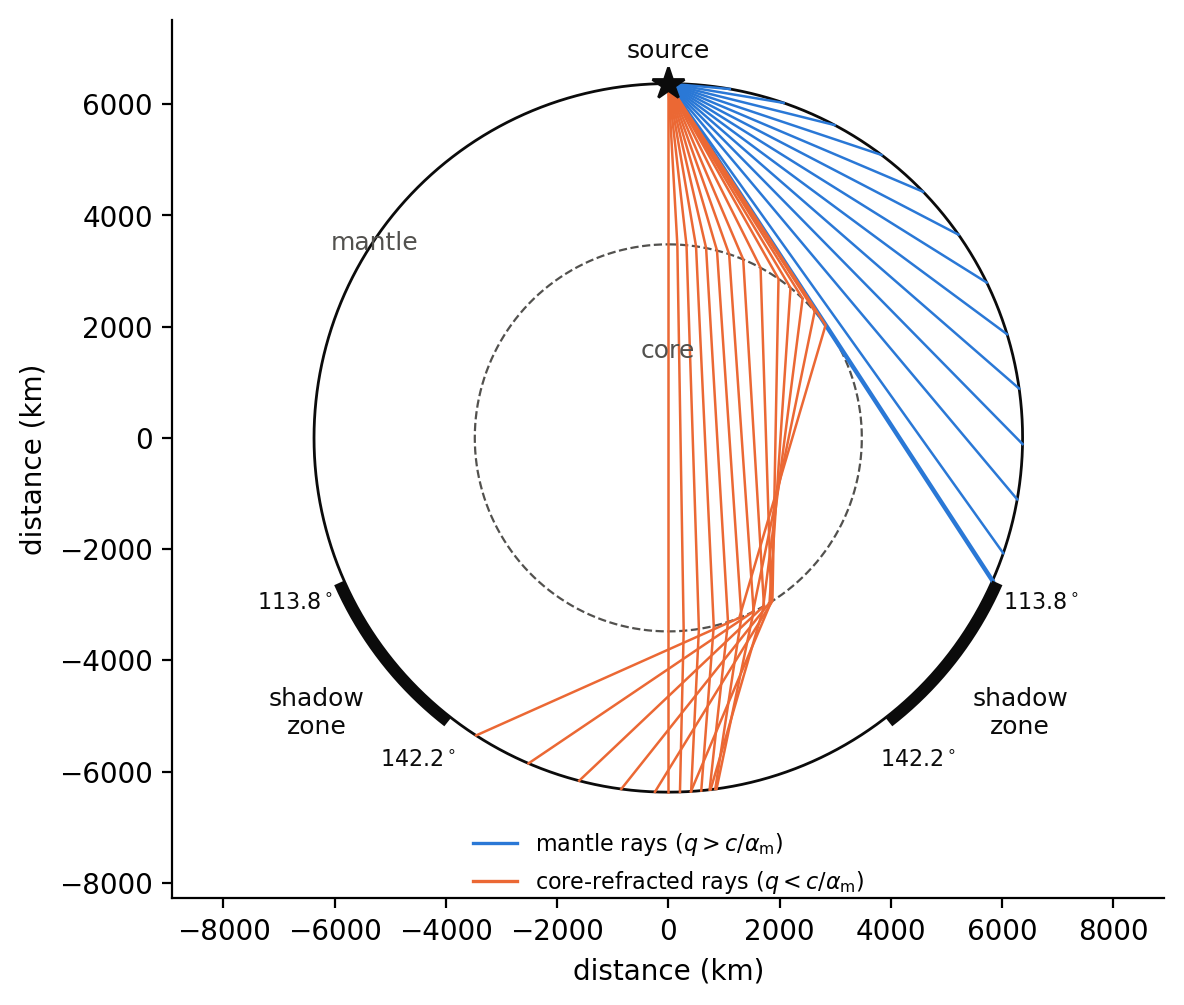
\includegraphics[width=0.7\textwidth]{figures_ex/ex6_shadow_zone.png}
\caption{Ray paths for a surface source in the two-layer model of Example~5. Mantle rays
(blue) are straight lines that emerge at distances up to $113.8^{\circ}$; rays that enter the
core (orange) are refracted towards the radial direction at the CMB and emerge no closer to the
source than $142.2^{\circ}$. The thick arcs mark the shadow zone on either side of the source.}
\label{fig:1}
\end{figure}

The far edge of the shadow zone agrees remarkably well with the observed value of
$142^{\circ}$, although this is partly fortuitous: in the real Earth it is set by the PKP
caustic rather than by the grazing ray, and its position depends on the details of the core
velocity structure. The near edge is predicted at $113.8^{\circ}$ rather than the observed
$103^{\circ}$ because the wave speed of the real mantle increases with depth. The mantle legs
of the grazing ray are then curved back towards the surface and each subtends less than
$\arccos(c/b)=56.9^{\circ}$, and the whole of Oldham's shadow zone moves closer to the source.
Within the shadow, seismograms are not silent: the core reflection PcP, waves diffracted
around the CMB, and S-waves and surface waves are all recorded there, but the sharp, direct
P-wave that dominates the first arrival at shorter distances is absent, and it was this
absence that led Oldham to infer the existence of the core.
\end{solution}

\end{document}
